% Overall overview of the adopted user testing procedure
\section{User Testing}

\subsection{General Method}
The core purpose of User Testing is to assess the usability properties of a system by observing how the system is used by users that are representative of real end users. It is a form of empirical research that aims to understand the relationship between humans and technology, learning how humans interact with a designed system through observed phenomena. 
Users are assigned pre-defined tasks to complete using the system and are then observed, recorded and finally analysed. 
Through user testing we can uncover actual difficulties that users will face, ones perhaps overlooked during the initial design of the system.

\subsection{Design Of The Study}
The User Testing study was designed to give probable users tasks that they would likely need to use the UNICEF website for. Moreover, as User Testing was performed after the Inspection testing of the website, the tasks were modelled to investigate further issues that were previously found. 

The user profile used for recruiting users was aimed at an age range of 20 to 35 as the average age of UNICEF volunteers is reported to be 34. Due to this age range’s familiarity with websites and technology in general, the tasks we designed to push their abilities.

After the initial inspection, it was discussed and agreed that the primary actions that a user can use the website for are:
\begin{itemize}
    \item To donate money 
    \item Research information
    \item Volunteer with the charity
    \item Find contact information
    \item Find the charity’s social media accounts
  \end{itemize}

  With each of these actions the quality of the site is not only tested by achieving the desired outcome for each task but also with what ease and efficiency can the user complete each action. 
  With each task the user is provided brief context and motivation for the action they need to preform. 

\begin{itemize}
    \item [A] Task: You would like to support UNICEF in their work. Make a once off donation of €10 euro to the charity. Warning, stop this task before confirming payment.

    \item [] Time Limit: 3 minutes

    \item [] Motivation: As UNICEF is a charity organisation, a primary goal of their website is to fundraise money. For this reason the action of donation is essential to the success of the website. 

    \item[B] Task: Your manager at work has a letter that must be sent to the ethic’s office of UNICEF. Find the appropriate postal address that this letter should be sent to
    
    \item [] Time Limit: 3 minutes 30 seconds

    \item[] Motivation: A primary action on a website of this kind is finding relevant contact information. After inspecting the website, we chose to ask for the Ethic’s Office postal address specifically as it’s location is not obvious, and so would be a greater test of our technologically apt test group. 

    \item[C] Task: From what you have read on the UNICEF website you are very interested in their work and you would like to be kept up to date with any news from the organisation. Find a way to subscribe to new information or updates from UNICEF

    \item [] Time Limit: 3 minutes 30 seconds

    \item[] Motivation: Getting users to subscribe to information updates is a useful tool for organisations such as UNICEF.
    
    \item[D] Task: You are interested in working with UNICEF either as an intern or as a volunteer. Find what opportunities are available
    \item[] Motivation: For a charity as large as UNICEF, finding new volunteers and employees is essential. We were also interested to see how users felt navigating these sections due to the large amount of information available. 

    \item [] Time Limit: 3 minute

    \item[E] Task: For a university project, you have been asked to write about the impact of charity work on Women’s Rights in Africa. You decide to do some research on the UNICEF website.
    Find out some information on the work the organisation does to help women in Africa. 
  
    \item [] Time Limit: 3 minutes 30 seconds
  
    \item[] Motivation: As already mentioned, a primary use of the website is for users to gather information on social issues and the work UNICEF does to help them. The task specified the information that needed to be found in order to see would users use the search feature or other methods. 

    \item[F] Task: You have recently become a parent. Find the area of the website with the relevant information about this topic and sign up.
    
    \item [] Time Limit: 4 minutes 15 seconds

    \item[] Motivation: This tas was chosen due to the action needing to be performed only being possible in one specific location. 
    
\end{itemize}

\subsection{Execution of The Study}

The testing was kept as uniform as possible across all users. With the exception of two users using the mobile version of the website and seven users doing the testing remotely. 

First the users were given an explanation of the testing with relevant guidelines and rules.  

Next the users were given a google form to fill out prior to starting the tasks. The form, shown below, recorded the user’s age, highest level education and some other general background data. The purpose of gathering this information is that it could possibly be later used to explain deviations in users’ success with the tasks.
\begin{figure}[h]
    \centering
    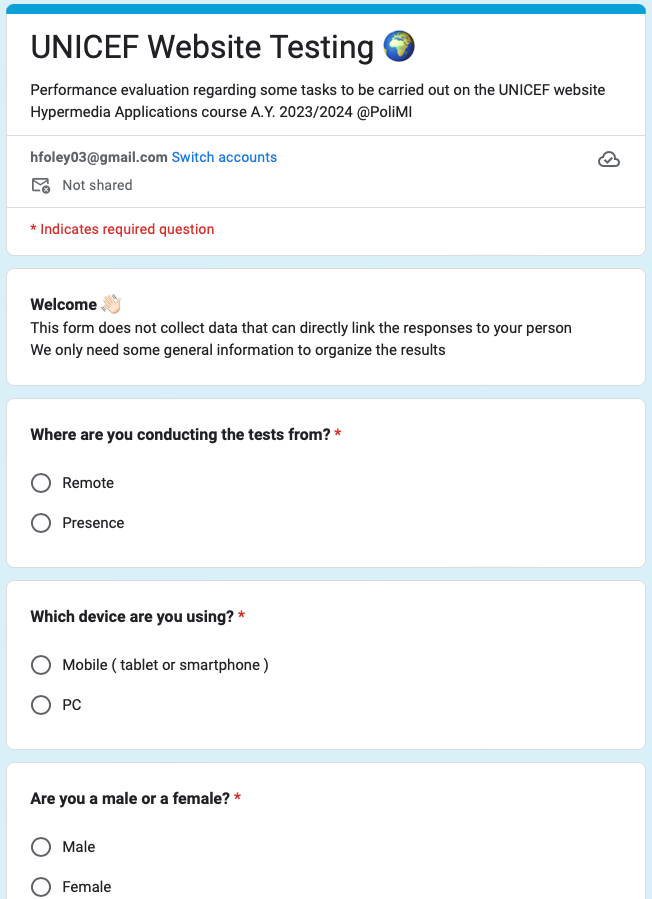
\includegraphics[scale=0.4]{Resources/Harry/GoogleForm.png}
    \caption{A section of the Google Form used for User Testing}
\end{figure}

It was decided to give minimal help to the users during testing to closer simulate the actual end user's experience.

A specific time limit was formulated for each task, with a user’s time exceeding this being considered a fail. However, users would not be told that they had failed a task if they exceeded the limit, as to not discourage them. This also allowed us to maximise the amount of information gathered during the study. The time limits were found through dummy testing with users not considered by the study. 

After the users had completed all tasks, they were asked to describe their experience, highlighting anything they found enjoyable or frustrating. 

\subsection{Results of User Testing}

To formulate our results from User Testing a Python script was written. This script took our data from an excel spreadsheet and created three charts. Two describing the profiles of the users, and one showing the completion times of each task. 
The two users that used a mobile device to complete testing were excluded from these results. 

\begin{figure}[h]
    \centering
    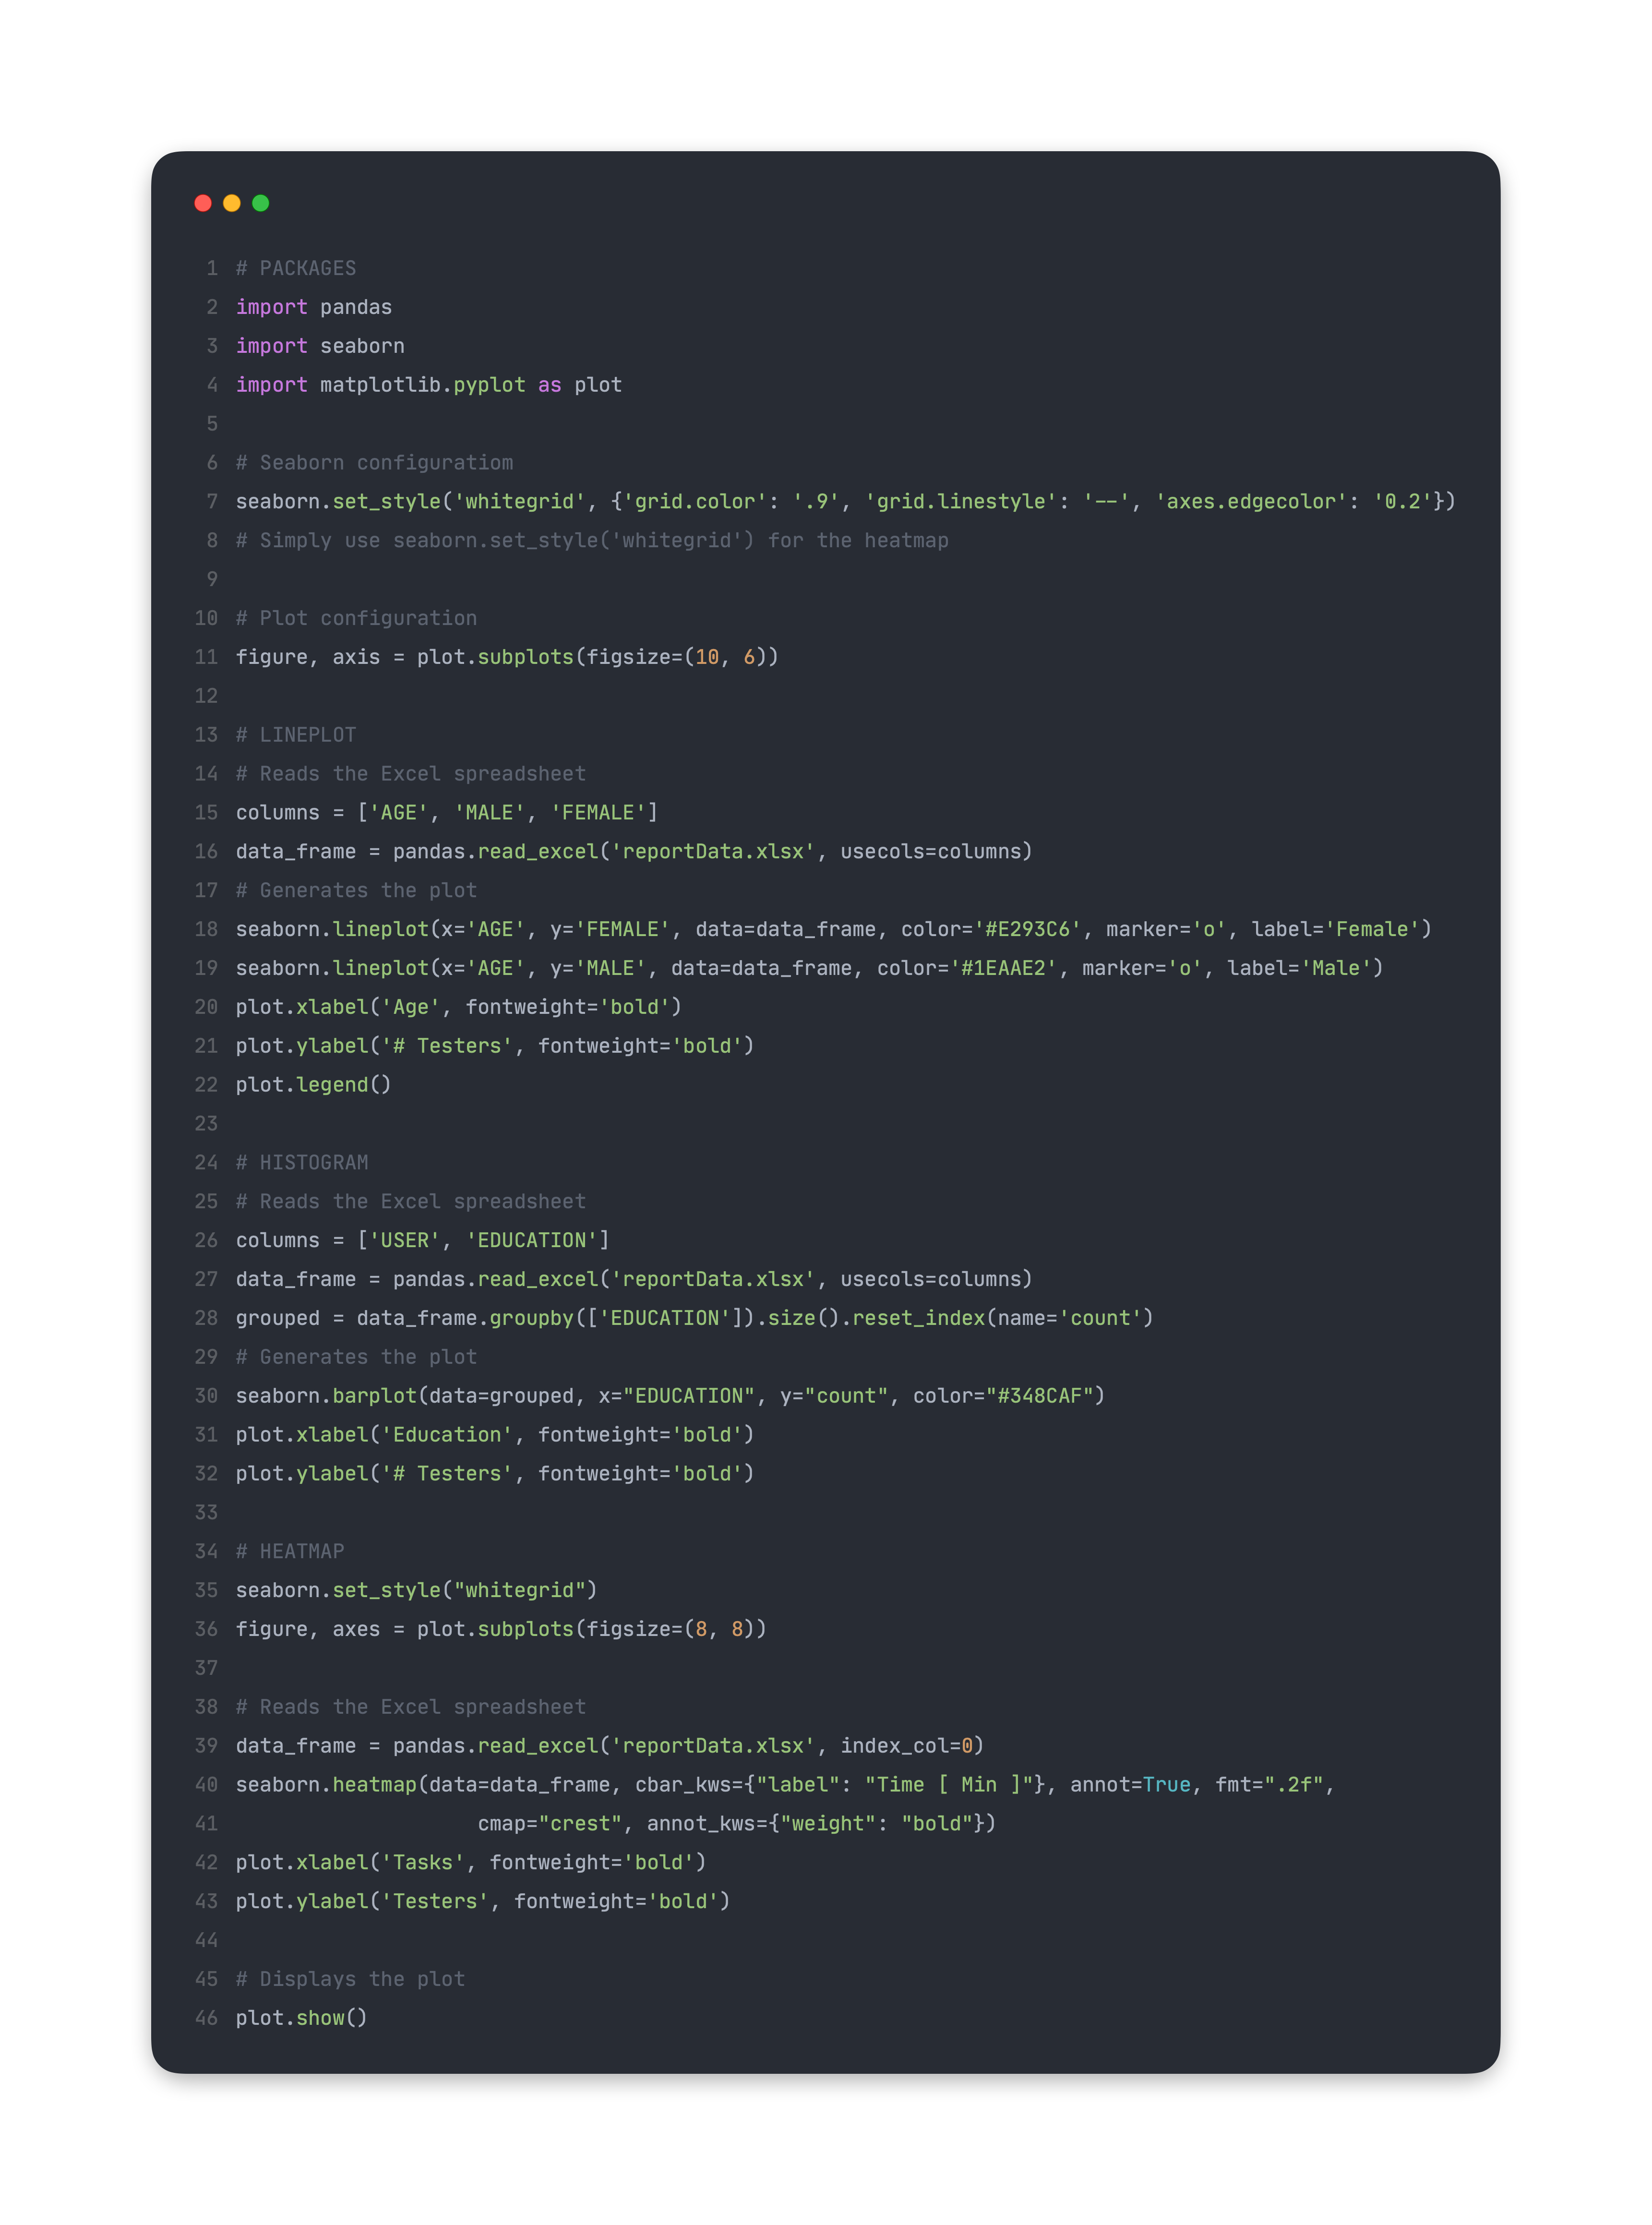
\includegraphics[scale=0.12]{Resources/Shared/pythonCode.png}
    \caption{Python Code used for User Testing Plots}
\end{figure}

In Figure 17 we can see the ages of the test group of 21 users. The majority of users were in the age range of 23 to 25, with only three users above the age of 25 and the oldest being 34. 
From the genders shown in this plot, we can see that the study had a balance of 10 males and 11 females.
  
\begin{figure}[h]
    \centering
    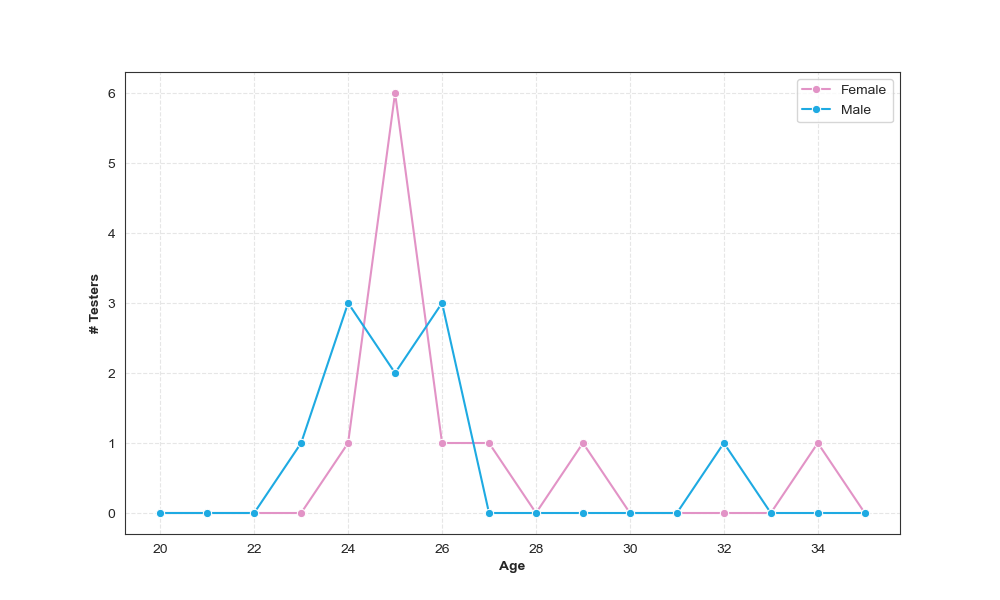
\includegraphics[scale=0.5]{Resources/Shared/agePlot.png}
    \caption{Age Plot from User Testing}
\end{figure}

Figure 18 shows the education background of the testers. All users were at university level. With 12 of 21 users self describing as being Master of Science students at university, this is the clear majority in our study. 
This followed by Bachelor of Science, with 5 users. 

\begin{figure}[h]
    \centering
    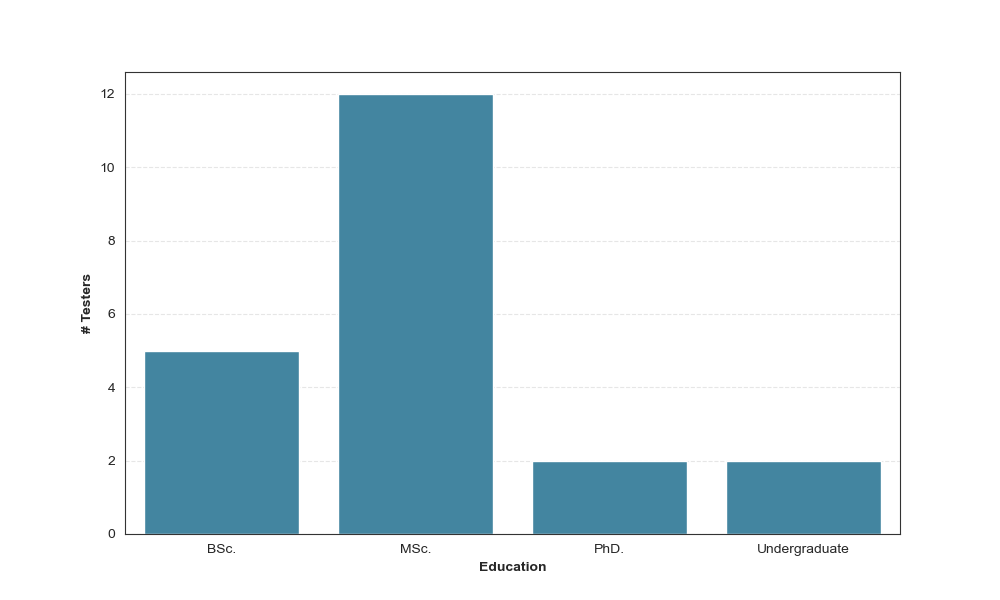
\includegraphics[scale=0.5]{Resources/Shared/educationPlot.png}
    \caption{Education Plot from User Testing}
\end{figure}

Finally, in Figure 19, we can see a plot showing each user's completion time of each of the six tasks. From this plot it is clear that most users managed to complete their tasks in a timely manner. This can be seen with the prominence of the light green colour, conveying completion times below two minutes.
However, it is also clear that there are a number of outliers, represented by the darker shades, showing that some users struggled with tasks and were slow in their completion.

\begin{figure}[h]
    \centering
    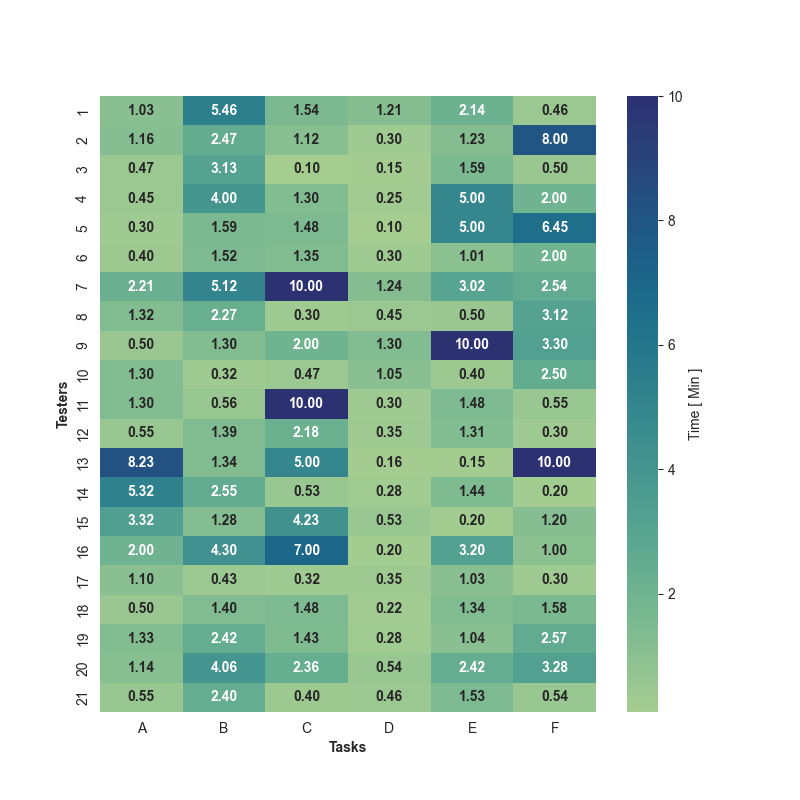
\includegraphics[scale=0.5]{Resources/Shared/taskstimePlot.png}
    \caption{User Testing Task Completion Times}
\end{figure}

\subsection{Discussion of Results}

Overall we are satisfied with the results generated through User Testing. The majority of users managed to complete the tasks below the time limits, with Task D being the only task that saw all users finishing below the target time.
Perhaps the most interesting observation lies in the outliers of the task completion times. In tasks A, C, E and F there were users who exceeded the time limit greatly, even though the majority of their peers completed the task in a timely fashion. 
This demonstrates to us that although the website is sufficient for most users there must be some improvements made in order to not discourage some users from using the website. 
This effect is seen strongest in Task F. The two quickest users found the sign up for Parenting Information in 30 seconds, but the slowest two users took 8 minutes and 11 minutes. 
This clearly shows that there are some flaws present in the design of the website.  

The list below outlines the most frequent comments from users after testing. 
\begin{itemize}
    \item Many testers found it difficult to navigate through the website, especially when trying to return to the homepage
    \item Several users expressed that they felt a sense of information overload using the site
    \item Users who used the site in Japanese and Chinese were unimpressed by the translations provided
\end{itemize}

These comments give greater context to the completion times. Even if the vast majority of users managed to complete their tasks within the time limit, the sentiment was not positive. 
Users overall described some operations as frustrating and difficult, with navigation and information overload being sticking points. 
It is also interesting that the users who chose to use the Japanese and Chinese language options of the website were displeased with their experience. As UNICEF is a highly international organisation, it is very important that they have inclusive language options to extend accessibility. 
